\documentclass[10pt,twocolumn,letterpaper]{article}

\usepackage{cvpr}
\usepackage{times}
\usepackage{epsfig}
\usepackage{graphicx}
\usepackage{amsmath}
\usepackage{amssymb}

% Include other packages here, before hyperref.

% If you comment hyperref and then uncomment it, you should delete
% egpaper.aux before re-running latex.  (Or just hit 'q' on the first latex
% run, let it finish, and you should be clear).
%\usepackage[pagebackref=true,breaklinks=true,letterpaper=true,colorlinks,bookmarks=false]{hyperref}

\cvprfinalcopy % *** Uncomment this line for the final submission

\def\cvprPaperID{****} % *** Enter the CVPR Paper ID here
\def\httilde{\mbox{\tt\raisebox{-.5ex}{\symbol{126}}}}

% Pages are numbered in submission mode, and unnumbered in camera-ready
\ifcvprfinal\pagestyle{empty}\fi

\newcommand\tab[1][1cm]{\hspace*{#1}}
\begin{document}

%%%%%%%%% TITLE
\title{CS-701 Final Report}

\author{Anowarul Kabir\\
George Mason University\\
{\tt\small akabir4@gmu.edu}
% For a paper whose authors are all at the same institution,
% omit the following lines up until the closing ``}''.
% Additional authors and addresses can be added with ``\and'',
% just like the second author.
% To save space, use either the email address or home page, not both
%\and
%Dr. Jana Kosecka\\
%George Mason University\\
%{\tt\small kosecka@gmu.edu}
}

\maketitle
\thispagestyle{empty}

%%%%%%%%% ABSTRACT
%\begin{abstract}
%this is my abstract
%\end{abstract}

%%%%%%%%% Introduction
\section{Introduction}
Object detection involves predicting class name as well bounding box of the object in the image. To do that, we need training images and their corresponding bounding box annotations. In this work, I have used state-of-the-art object detection networks called Faster R-CNN\cite{NIPS2015_5638}. It predicts objects with an objectness score from an image using region proposals generated by regional proposal network. To train and test the model, I have used a fine-grained dataset, where classes are involved in subcategories of the class, called Cats and Dogs\cite{parkhi12a}.

In the next phase, I have worked in few shot classification regimes where samples are very limited in number. Humans have shown very high degree of accuracy in classifying object even when only one example is available. To do this job I have used prototypical networks\cite{DBLP:journals/corr/SnellSZ17}, which basically calculate prototype representation for each class; and then by measuring distance from the query points to that prototypes it predicts classes. To do that I have used Omniglot\cite{DBLP:journals/corr/abs-1902-03477} dataset.

%%%%%%%%% Methodology
%\section{Methodology}
%The work is divided into two parts. First task is involved in object detection using Faster R-CNN and second one %is the classification task using prototypical networks in in few-shot regime. 

\section{Faster R-CNN}
Faster R-CNN comprises of Regional Proposal Network (RPN) and a detector network. RPN produces region proposals with an objectness score by taking feature maps as an input. The feature maps are generated by the feature extractor. Finally, the detector network takes the region proposals as input and outputs class name with bounding box prediction. The whole system is single and unified for object detection. 

RPN takes feature map of an image which is extracted by the feature extractor. Feature extractor comprises of multiple convolutional layers, activation layes and subsampling layers. The feature maps maintain some statistical relationship e.g. spational relation among pixels, channelwise relationship etc. RPN is the fully convolutional networks that predicts object bounds and objectness score at each position, each generates high quality region proposals. RPN and fast rcnn share convolutional features using attention mechanism. RPN is designed to efficiently predict region proposals with a wide range of scales and aspect ratios. In one sentence, RPN takes an image of any size as input and outputs a set of rectangular obj proposals, each with objectness score. There are three ways to handle multiple scales and aspect rations of the image. 1) Pyramids of images and feature maps, and the classifier will run on all scales. It is time consuming. 2) Pyramids of filters with multiple scales and aspect rations, will run on all feature maps. 3) Pyramids of reference boxes, called anchors, that serve as multiple scales and aspect rations. This paper laverages the anchor mechanism. \cite{NIPS2015_5638}

RPN works as a sliding window fashion. First, they slide a small network over the convolutional feature map. This small network takes nxn spatial window of the convolutional feature map as input. Each sliding window is mapped to a lower-dimensional feature. This feature is then fed into two fully connected layers - a box regression layers and a box classification layer. At each sliding-window location, we predint at most k region proposals. The regression layer has 4k outputs which stands for bounding box coordinates for k boxes. The classification layer has 2k outputs which estimates the probability of object or not object for each proposal. These k reference boxes are called anchors. For each anchor we assign binary class label (object or not object). Then we assign positive label to two kinds of anchors- 1) Anchors with the highest IoU overlap with the ground truth box. 2) Anchors with IoU overlapp value higher than 0.7 with ground truth box. Then we assign negative label to a non-positive anchor if IoU ratio is lower that 0.3 for all groud truth box. Anchors that are neither positive nor negative do not contribute to the training objective. \cite{NIPS2015_5638}

In the training scheme, we fine-tune for the region proposal task or fine-tune for the object detection task while keeping the proposals fixed. The training process named alternating training involves four steps. 1) Train the RPN and fine-tune if for the the region proposal task. 2) Then train the separate detection network by Fast R-CNN using the proposals generated by RPN. 3) We use the detector network to initialize RPN training, but we fix the shared convolutional layers and fine-tune the layers unique to RPN. 4) Finnally, keeping the shared convolutional layers fixed, we fine tune the unique layers of the fast R-CNN. At this point, both RPN and Fast R-CNN are sharing same convolutional layers. \cite{NIPS2015_5638}

The loss function \cite{NIPS2015_5638} is calculated over two loss function. We calculate the log-loss over two clssses (object or not object) and sum them up and then normalize the score. Then we calculate the $L_1-smooth$ loss over the predicted bounding box coordinates and ground-truth bounding box coordinates, sum them up and normalize the score. The final loss function is calculated by the following equation:
\begin{equation}
\begin{split}
L(\{p_i\}, \{t_i\}) = \frac{1}{N_{cls}} \sum_i L_{cls}(p_i, p_{i}^*) \\
                        + \lambda \frac{1}{N_{reg}} \sum_i p_{i}^* L_{reg}(t_i, t_{i}^*)
\end{split}
\end{equation}

Here, $i$ is an index of an anchor in a mini-batch. $p_i$ is the predicted probability of an anchor $i$ being an object. $p_{i}^*$ is the ground-truth label and value of this is $1$ and $0$ if the anchor is positive and negative respectively. $t_i$ is predicted bounding box and $t_{i}^*$ is the ground-truth bounding box associated with a positive anchor. $L_{cls}$ is the log-loss over two classes (object or not object) and $L_{reg}$ is the $smooth-L1$ loss over predicted bounding box and ground-truth bounding box. $\{p_i\}$ and $\{t_i\}$ are the outputs of the classification and regression layers. Finally, $N_{cls}$ is the mini-batch size and $N_{reg}$ is the number of anchor locations in an image.

\section{Prototypical Networks for Few-shot Learning}
Humans have shown the ability of high degree of accuracy in performing classification when involved in very few examples even one example per class. In few-shot classification, the classifier must generalize to new classes given only a small number of examples of each class. Prototypical networks[] learn a metric space in which classification can be performed by computing distances to prototype representation of each class. The prototypical networks learn a non-linear mapping of the input into an embedding space using neural network and take the class prototype to be the mean of its support set in the embedding space. Classification is then performed for an embedded query point by simply finding the nearest class prototype. \cite{DBLP:journals/corr/SnellSZ17}

The training episode involves two parts: 1) Computing prototypes 2) Loss calculation. To compute prototypes, representatives for each class, we first randomly select a set of classes($N_c$) from the traing set where we have all $K$ classes. Then for each classes ($k in N_c$) we randomly sample a support set ($S_k$) and a query set ($Q_k$). Then we compute prototype($c_k$) for each classes by
\begin{equation}
c_k=\frac{1}{|S_k|}\sum_{(x_i, y_i) \epsilon S_k} f_{\phi}(x_i)
\end{equation}
where $x_i \epsilon R^D$ is $D$ dimensional feature vector and $y_i \epsilon \{1, 2,...,K\}$ is the corresponding label. And $f_\phi$ is the embedding function, $f_\phi : R^D \to R^M$ with learnable parameters $\phi$. Then we calculate and update the loss function using following equation:
\begin{equation}
\begin{split}
J=J+\frac{1}{N_c N_Q}[d(f_\phi(x), c_k) \\
                     +log \sum_{k'}exp(-d(f_\phi(x), c_{k'}))]
\end{split}
\end{equation}
where, $d$ is the euclidean distance between a prototype and a sample($x$) from query set($Q_k$).

\section{Result}
This section is divided into two parts. First part shows the result on object detection over Cats and Dogs\cite{parkhi12a} dataset. And the second part shows the result on prototypical networks over Omniglot dataset\cite{DBLP:journals/corr/abs-1902-03477}.

\subsection{Results on Object Detection}
I have used Cats and Dogs\cite{parkhi12a} dataset for training and testing the pet detector. The dataset is basically fine grained datset, which involves subcategories of a class. In our case, we have in total 37 classes. I have also extented the dataset by adding one cat class named "Savannah". So in extended dataset there are 38 classes. The dataset involving new class is collected from different websites. After collecting dataset, I have used GNU Image Manipulation Program (GIMP) for annotating tight bounding box over the head of the image as a ground-truth bounding box. I have also used GIMP to annotate the trimap (0 for cat, 1 for background and 2 for others or boundary).\\\\
Dataset statistics:\\
	\tab- 37 classes (Cat: 12, Dog: 25)\\
	\tab- Train set: 2208 images\\
	\tab- Validation set: 552 images\\
	\tab- Test set: 920 images\\
Extended Dataset statistics:\\ 
	 \tab- 38 classes (Cat: 13, Dog: 25)\\
	 \tab- Train set: 2328 images\\
	 \tab- Validation set: 582 images\\
	 \tab- Test set: 970 images\\
	 \tab- Newly added 200 images\\

The results on two datasets over different mean average precision (mAP) with intersection over union (IoU) have shown in Table 1 and Table 2.

\begin{table}[h]
\begin{tabular}{ |p{1.5cm}||p{1cm}|p{1cm}|p{1cm}|p{1cm}|  }
 \hline
 \multicolumn{5}{|c|}{Results on Pet Dataset} \\
 \hline
 Set & Images & mAP@ IoU= 0.5:0.95 & mAP@ IoU= 0.5:0.95 &mAP@ IoU= 0.5:0.95 \\
 \hline
 Validation & 552 & .705 & 0.875 & 0.831 \\
 \hline
 Test & 920 & 0.706 & 0.908 & 0.853 \\
 \hline
\end{tabular}
\caption{mAP@IoU on pet dataset}
\end{table}

\begin{table}[h]
\begin{tabular}{ |p{1.5cm}||p{1cm}|p{1cm}|p{1cm}|p{1cm}|  }
 \hline
 \multicolumn{5}{|c|}{Results on Extented Pet Dataset} \\
 \hline
 Set & Images & mAP@ IoU= 0.5:0.95 & mAP@ IoU= 0.5:0.95 &mAP@ IoU= 0.5:0.95 \\
 \hline
 Validation & 582 & 0.718 & 0.907 & 0.853\\
 \hline
 Test & 970 & 0.712 & 0.912 & 0.849\\
 \hline
\end{tabular}
\caption{mAP@IoU on extended pet dataset}
\end{table}

To have a general idea of inference, I have taken randomly 20 images per class. The two images below are showing how many images are correcly and incorrectly predicted by the green and red line respectively.

\begin{figure}[h]
\caption{Inference out of 20 images}
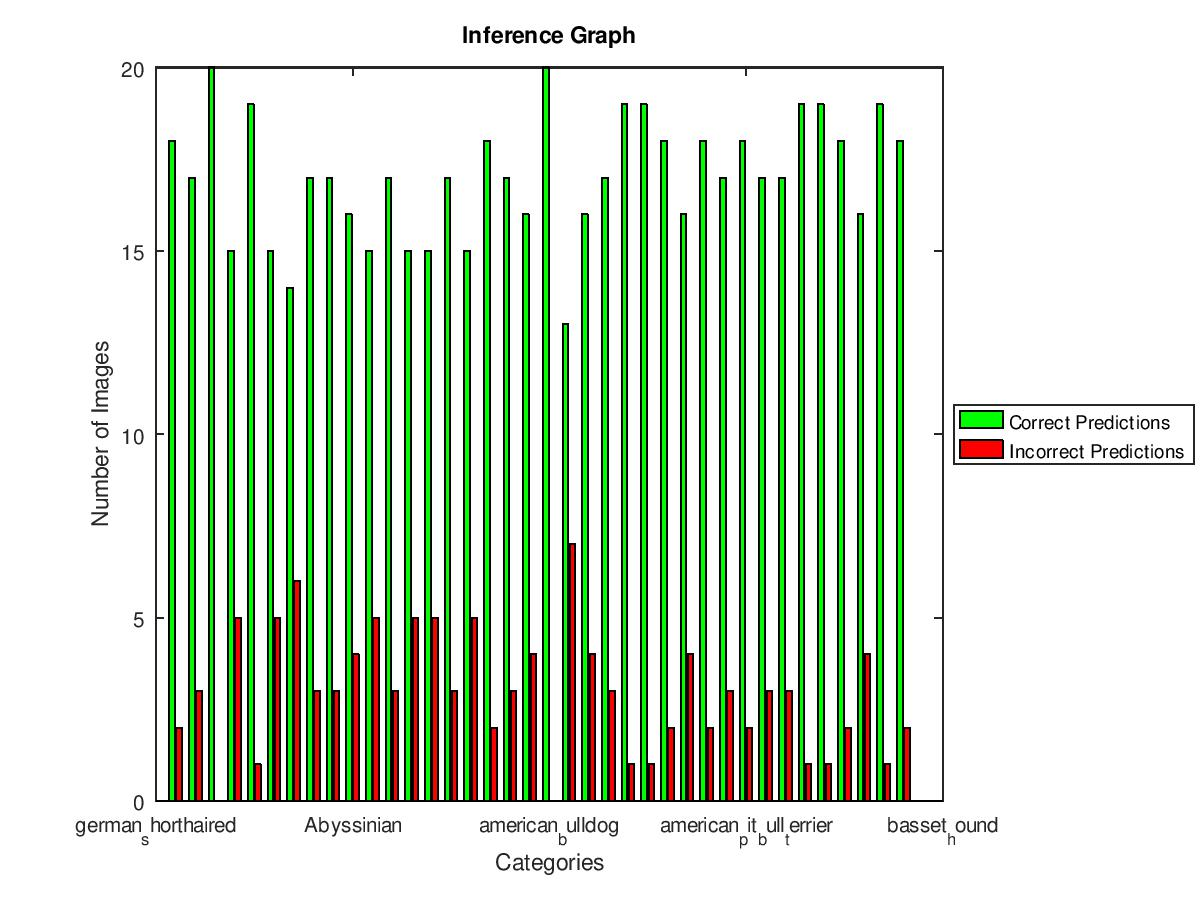
\includegraphics[width=8cm]{images/inference_bar_plot.jpg}
\centering
\end{figure}

\begin{figure}[h]
\caption{Inference out of 20 images}
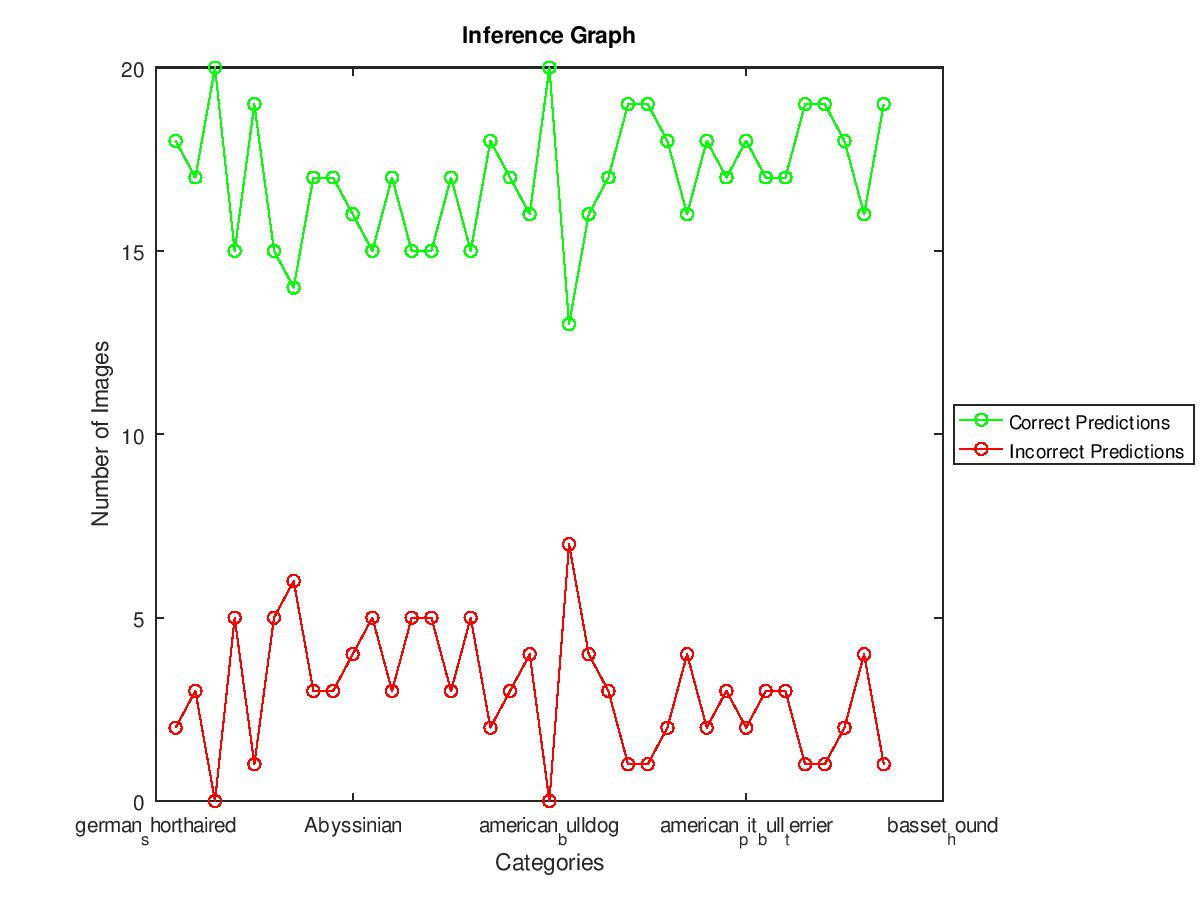
\includegraphics[width=8cm]{images/inference_scatter_plot.jpg}
\centering
\end{figure}

\subsection{Results on Few-shot Classification}
I have used Omniglot\cite{DBLP:journals/corr/abs-1902-03477} dataset to train and validate the images using prototypical networks. The accuracy and loss at train and validation time are shoing on Table 3.

\begin{table}[h]
\begin{tabular}{ |p{1.5cm}||p{2cm}|p{1cm}|p{1cm}|  }
 %\hline
 %\multicolumn{4}{|c|}{Results on Omniglot Dataset} \\
 \hline
 Set & Output Proces & Accuracy & Loss \\
 \hline
 Train & 60-way 5-shot & 0.994 & 0.012 \\
 \hline
 Validation & 60-way 5-shot & 0.990 & 0.024\\
 \hline
\end{tabular}
\caption{Results on Omniglot Dataset}
\end{table}

In Figure 3 and Figure 4, it is showing accuracy/loss versus time graph using greet and red points.

\begin{figure}[h]
\caption{Accuracy/Loss vs. Time at train}
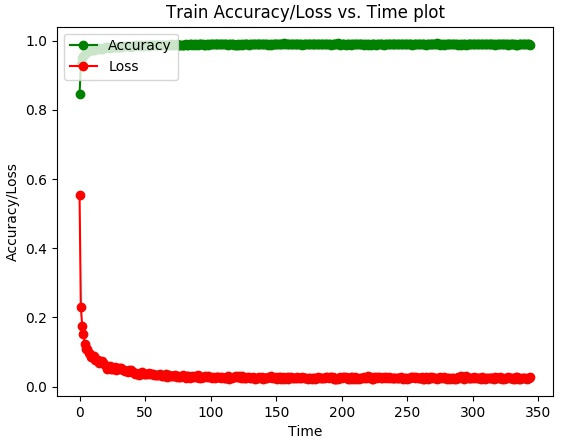
\includegraphics[width=8cm]{images/train_omniglot_acc_loss_plot.jpg}
\centering
\end{figure}

\begin{figure}[h]
\caption{Accuracy/Loss vs. Time at validation}
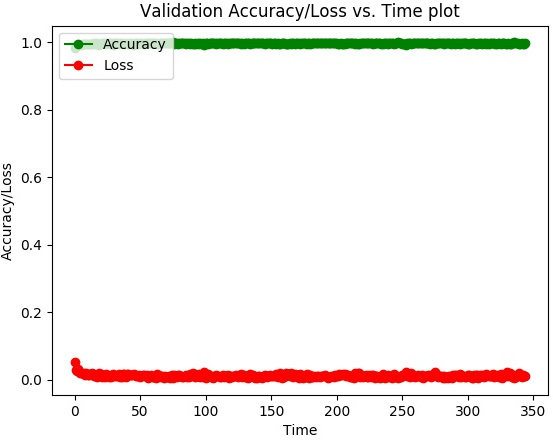
\includegraphics[width=8cm]{images/val_omniglot_acc_loss_plot.jpg}
\centering
\end{figure}
 

%%%%%%%%% References
{\small
\bibliographystyle{ieee}
\bibliography{report}
}
\end{document}